\chapter{Visualização de Software}\label{chap:visualizacao}

Na primeira parte deste trabalho, investigamos algumas técnicas de visualização
de software, como primeira abordagem para melhor a apresentação dos valores das
métricas no Mezuro. Isso porque, a visualização de um dado com propriedades
visuais como posição, tamanho, forma e cor, potencializam as habilidades
sensoriais do ser humano. Possivelmente o usuário irá extrair observações e
conclusões sobre os dados, e também poderá moldar esse conhecimento adquirido
para atingir os objetivos \cite{card1999readings} \cite{heer2012interactive}
\cite{keim2002information}.

O estudo da visualização pode ser dividido em duas grandes vertentes, ambas
possuindo interação com usuário induzindo-o ao entendimento das informações
contidas nos dados \cite{de2003visual}:

\begin{enumerate}
  \item \textbf{Visualização Científica}: dados físicos e inerentemente
  geométricos;
  \item \textbf{Visualização de Informação}: informações não físicas, por
  exemplo coleções de documentos, podem ser beneficiadas, porém não há nenhuma
  forma óbvia de se mapear tais dados em uma imagem \cite{card1999readings}.
  Envolve algo mais complexo.
\end{enumerate}

Visualização da informação é portanto relacionada a \textbf{grandes conjuntos}
de dados. Um \textbf{conjunto} é um o número de atributos ou dimensões que o
identifica. Quantidade de dimensões é o mesmo que \textbf{dimensionalidade}.

Os tipos de dados comuns são: bidimensionais e multidimensionais
\cite{de2003visual}.

Os multidimensionais necessitam da aplicação de uma técnica
\cite{keim2002information}. São técnicas citadas por \citeonline{messias2012}:

\begin{itemize}
  \item Projeções geométricas:
	\begin{itemize}
		\item Coordenadas paralelas. Exemplo na Figura \ref{fig:parallel} \cite{kaichang2015};
	\end{itemize}
  \item Orientadas a pixel:
	\begin{itemize}
		\item \textit{recursive patterns};
		\item \textit{circle segments};
	\end{itemize}
  \item Iconográficas:
	\begin{itemize}
		\item \textit{stick figures};
	\end{itemize}
  \item Hierárquicas:
	\begin{itemize}
		\item \textit{Dimensional Stacking}.
	\end{itemize}
\end{itemize}

\begin{figure}[!htb]
  \centering
    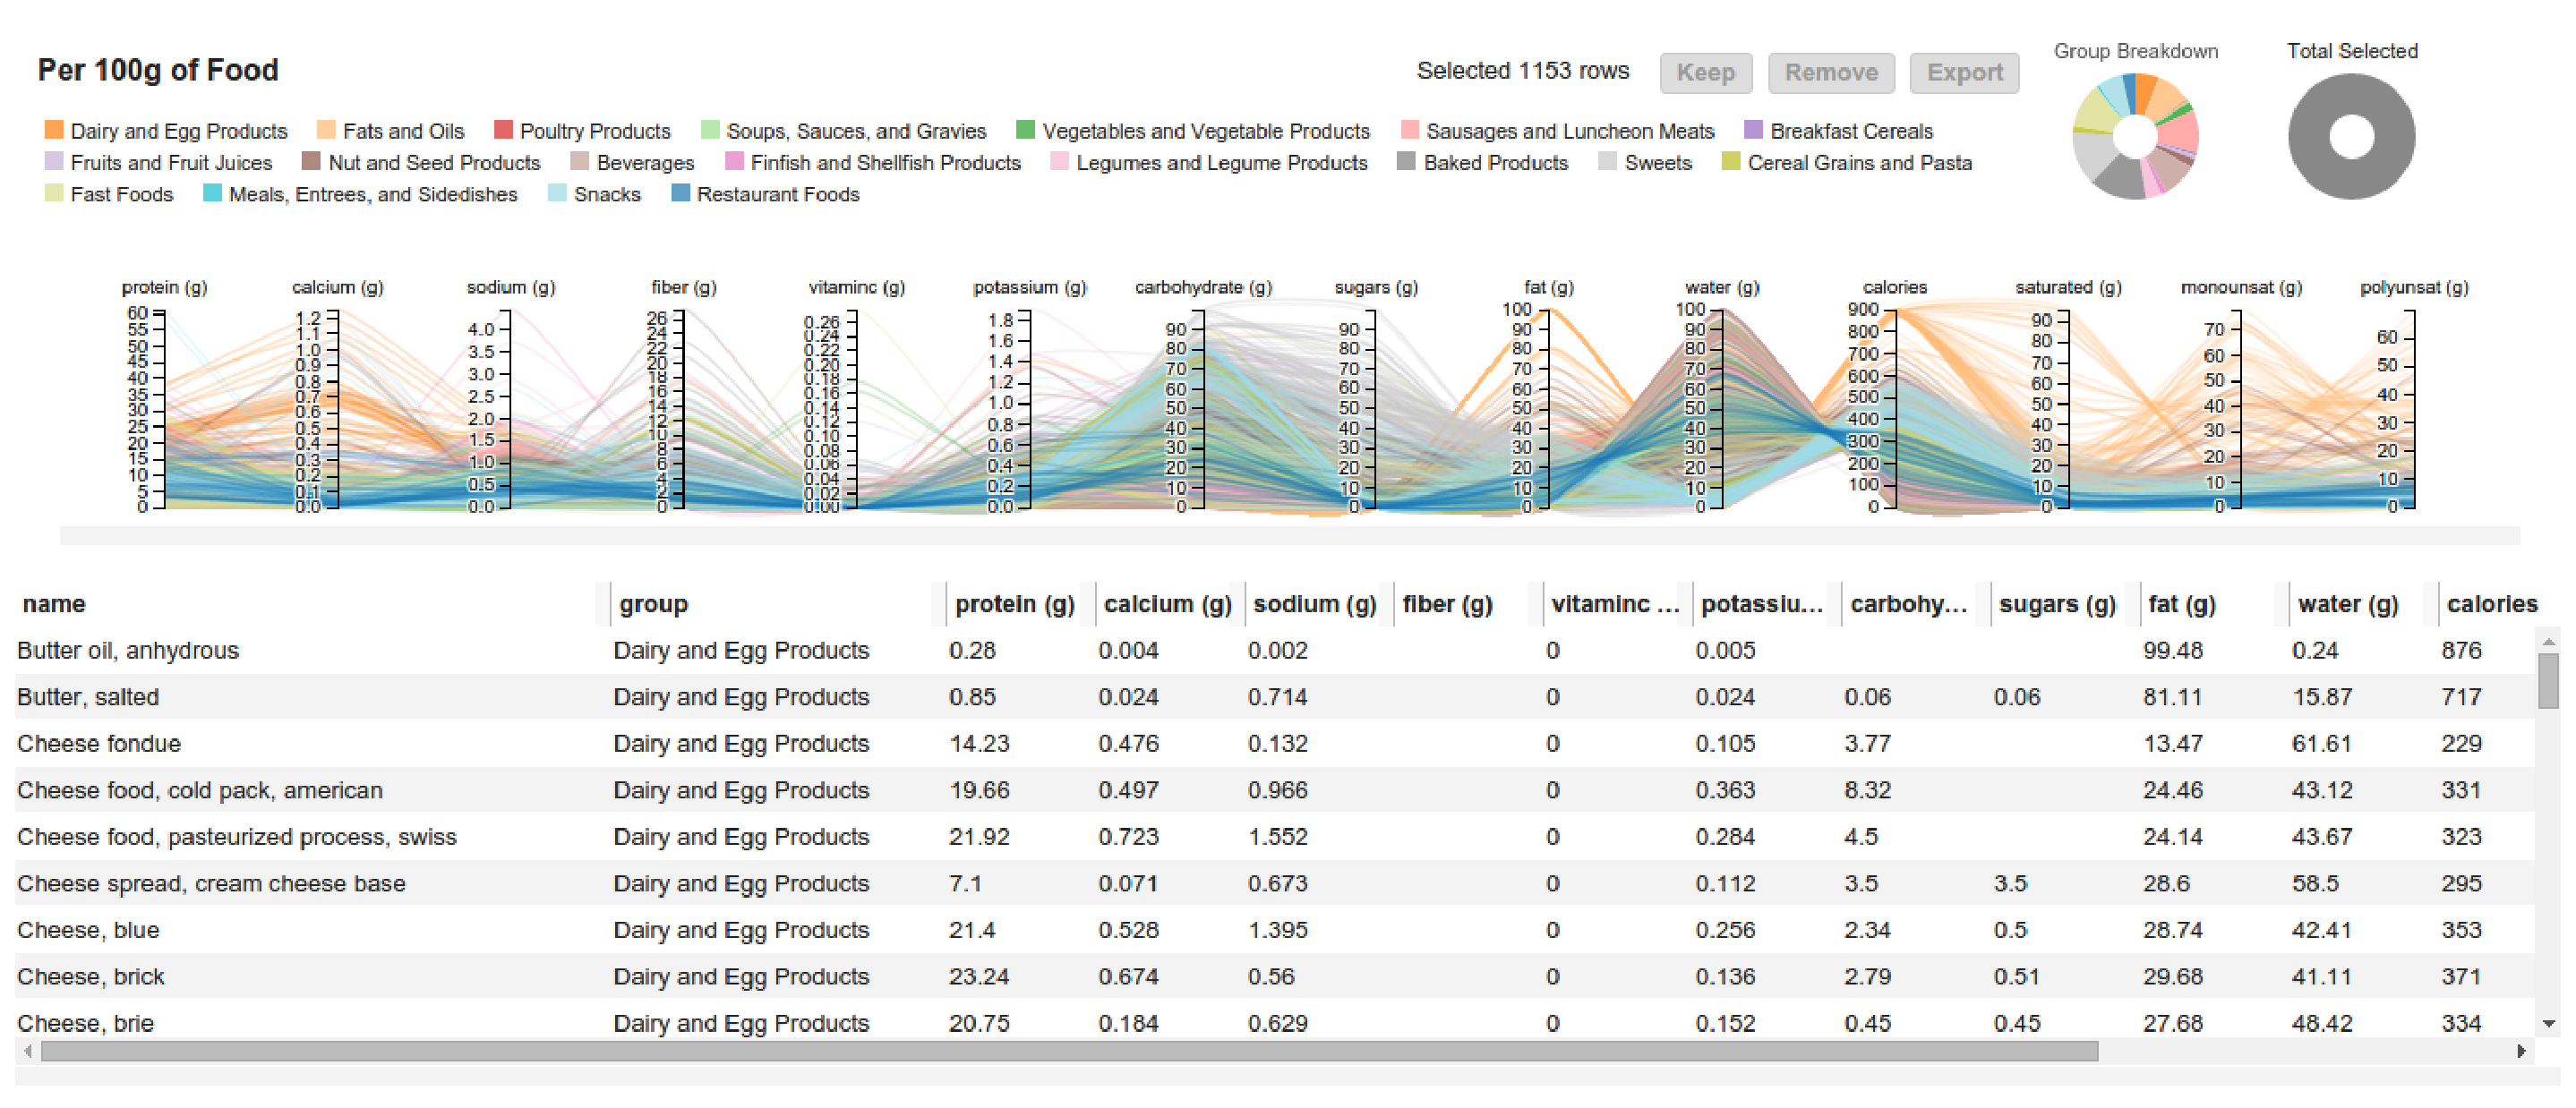
\includegraphics[keepaspectratio=true,scale=0.3]
    {figuras/parallel.eps}
  \caption{Exemplo de Coordenadas Paralelas}
  \label{fig:parallel}
\end{figure}

Portanto, segundo \citeonline{diehl2007software}, Visualização de Software
é uma subárea da Visualização de Informação. E os objetivos dela são: ``auxiliar
a compreensão de sistemas complexos de software e melhorar a produtividade do
processo de desenvolvimento'' \cite{messias2012}. É a representação gráfica de
aspectos técnicos, ou sociais, ou ambos de um software. As técnicas geram
exibições de aspectos do software que podem auxiliar tarefas de:

\begin{itemize}
	\item Gerenciamento;
	\item Projeto;
	\item Implementação;
	\item Depuração;
	\item Análise;
	\item Manutenção.
\end{itemize}

Visualização de Software é um dos braços da Visualização de Informação que mais
cresce \cite{telea2014data}. \citeonline{bassi2001software} apresentam alguns
benefícios de se utilizar ferramentas de VS:

\begin{itemize}
	\item Economia de tempo e dinheiro;
	\item Melhor compreensão;
	\item Aumento da produtividade;
	\item Auxílio na detecção de erros no código;
	\item Melhoria da qualidade.
\end{itemize}

\section{Categorias da Visualização de Software}

A visualização de software pode ser levada em consideração pelas três seguintes
categorias: estrutura, comportamento e evolução \cite{diehl2007software}.

\subsection{Estrutura}

Relacionada ao que é estático em um software, sem necessidade de executá-lo. Por
exemplo: o código-fonte, as estruturas de dados do programa, o grafo de chamadas
estático e a organização do sistema em módulos \cite{diehl2007software}.

Propriedades interessantes \cite{messias2012}:

\begin{itemize}
	\item Exatidão: linguagens de programação exacerbadamente definidas;
	\item Grande escala: sistemas que possuem uma quantidade grande de linhas
	de código;
	\item Relações e hierarquias entre entidades do código;
	\item Diversos atributos que expressam as características dessas entidades.
\end{itemize}

Ferramentas de geração de visualização da categoria estrutura compartilham o
mesmo modelo conceitual: a geração de um grafo que relaciona em seus vértices
as propriedades anteriormente citadas.

Exemplos de Visualização da estrutura de software: \textit{Team Assessment}
\cite{telea2009case} e \textit{CodeCity} \cite{wettel2008codecity}.

Uma técnica bastante elaborada, desenvolvida por \citeonline{holten2006hierarchical},
expressa em uma única imagem duas das propriedades: a estrutura hierárquica e
suas dependências internas (Figura \ref{fig:heb}).

\begin{figure}[!htb]
  \centering
    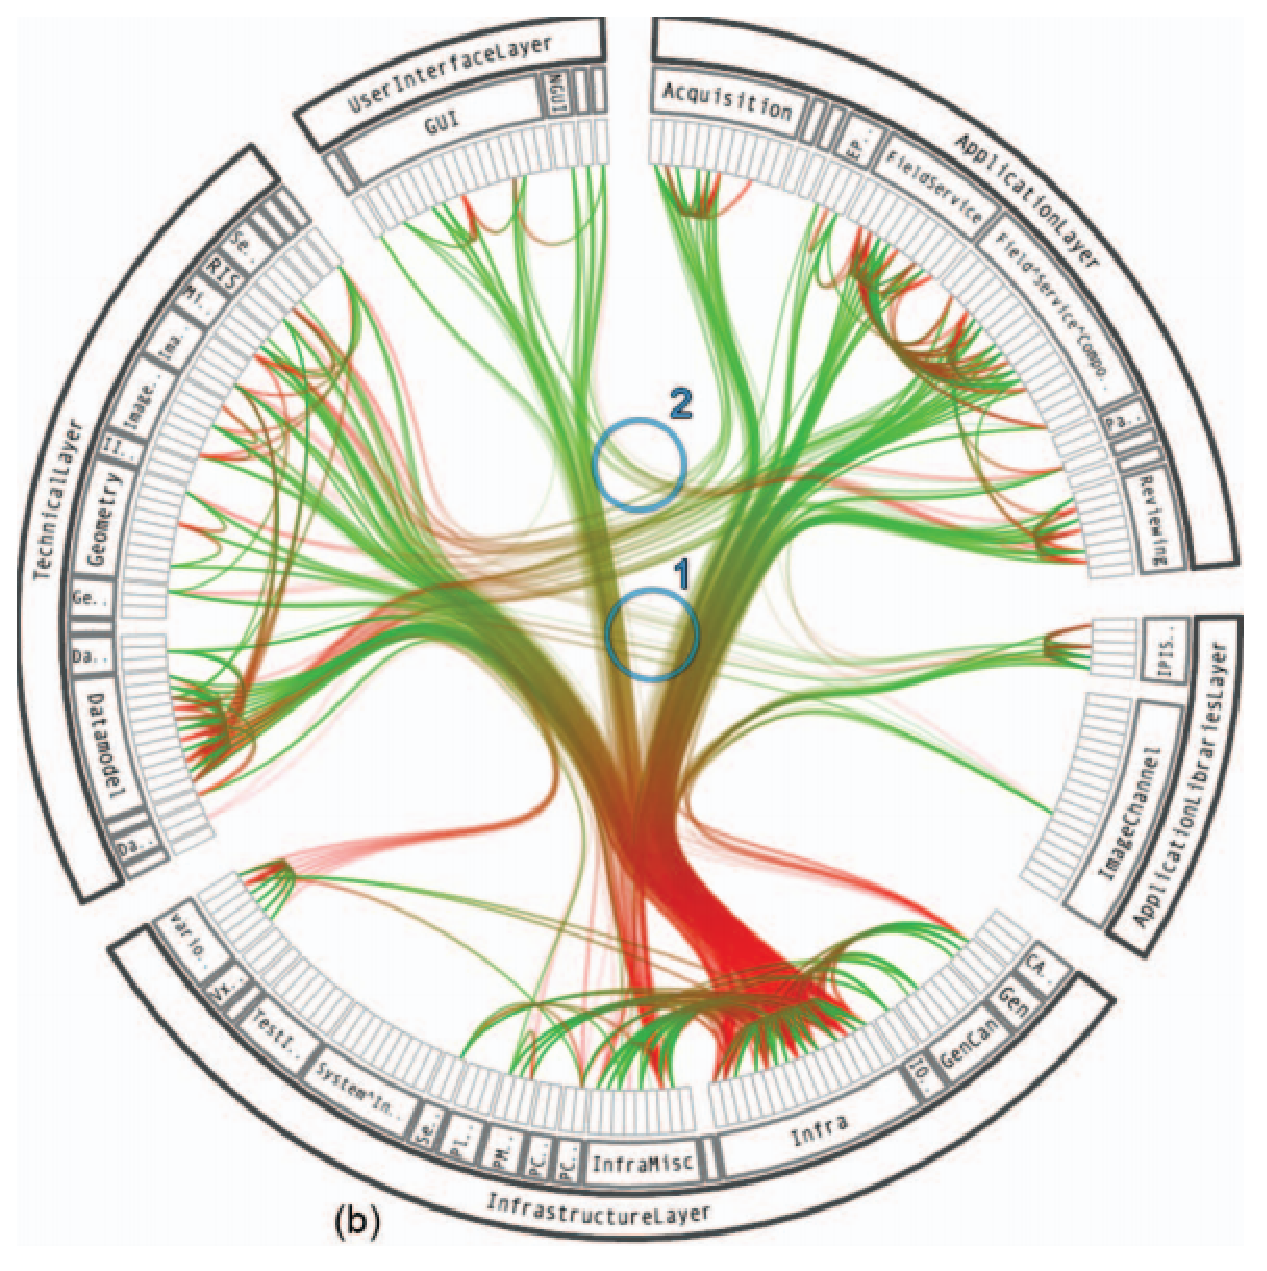
\includegraphics[keepaspectratio=true,scale=0.5]
    {figuras/heb.eps}
  \caption{Estrutura Hierárquica \cite{holten2006hierarchical}}
  \label{fig:heb}
\end{figure}

Métricas podem ser incluídas em visualizações da estrutura. Na ferramenta
SolidSX (Figura \ref{fig:solidSX}), \citeonline{reniers2011visual} inclui
algumas métricas como linhas de código, comentários e complexidade. Essa
ferramenta une três técnicas:

\begin{itemize}
	\item \textit{TreeMap} - disposição das hierarquias do código;
	\item \textit{HEB};
	\item \textit{TableLens} - módulos são linhas e métricas são colunas de uma
	tabela, mapeando as métricas e destacando-as por cores.
\end{itemize}

\begin{figure}[!htb]
  \centering
    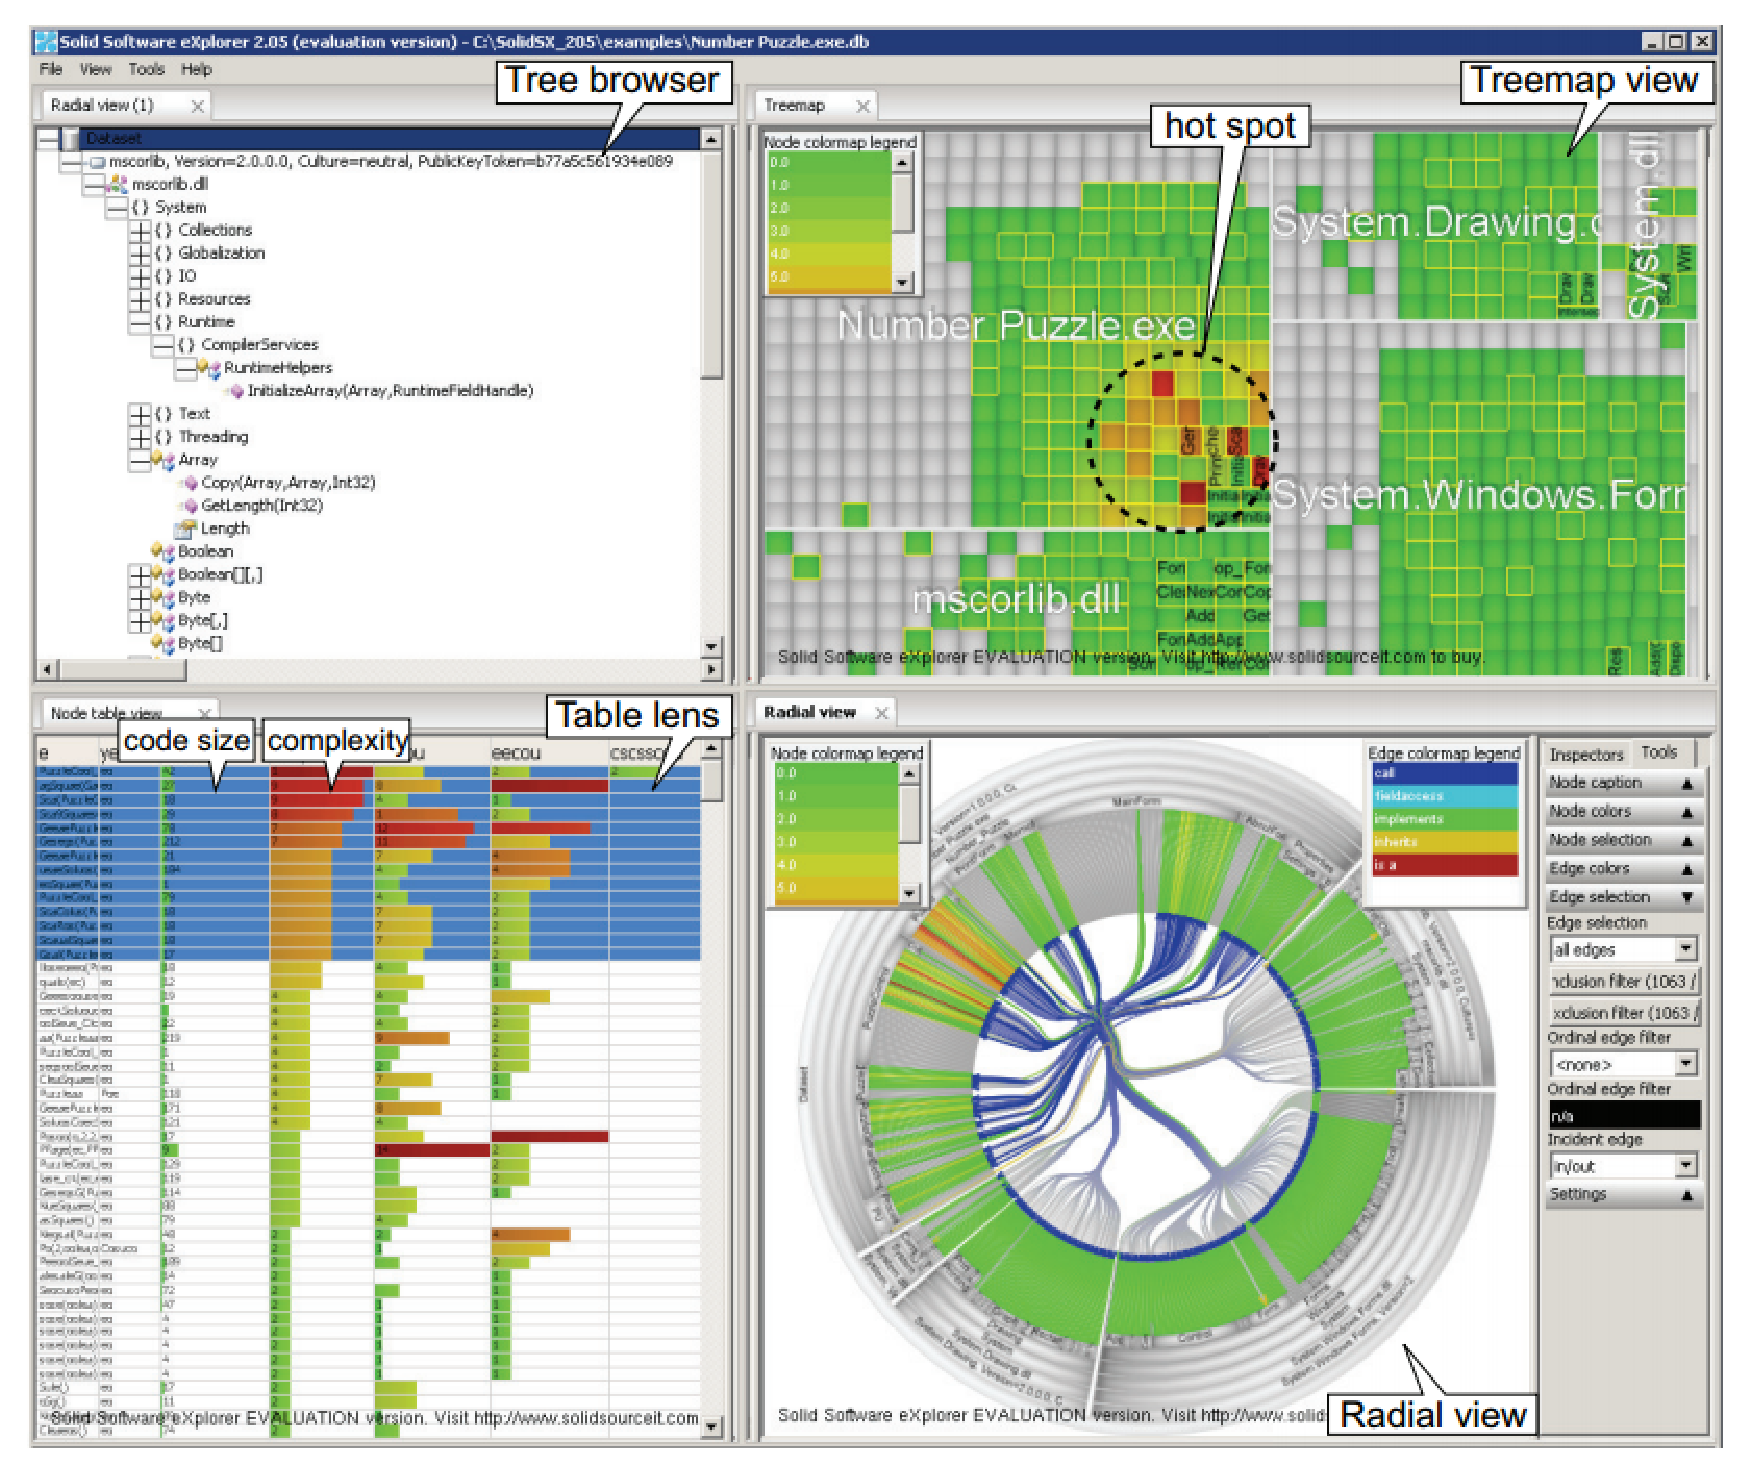
\includegraphics[keepaspectratio=true,scale=0.5]
    {figuras/solidSX.eps}
  \caption{Ferramenta SolidSX \cite{reniers2011visual}}
  \label{fig:solidSX}
\end{figure}

\subsection{Comportamento}

Nesta categoria o software é executado. Análise do que acontece, em tempo de execução, dada
determinada entrada. Técnica: sequência de estado. Combinar dados e código para
analisar interação com a memória. Dependendo do paradigma de programação, pode
haver uma relação entre os métodos ou funções e a comunicação entre os objetos
\cite{cornelissen2009systematic} \cite{diehl2007software}.

Aplicações dessa categoria:

\begin{itemize}
	\item Análise de traces de execução;
	\item Visualização dinâmica e recuperação de arquitetura;
	\item Animação de algoritmos;
	\item Depuração visual;
	\item Apoio visual à atividade de teste.
\end{itemize}

Exemplo da ferramenta \textit{Tarantula} \cite{jones2002visualization} -
Depuração visual, execução de testes, destaque com escala que vai de vermelho
(falha) até verde (sucesso).

\subsection{Evolução}

Categoria aplicada para compreensão das modificações ao longo do tempo. A
manutenção e evolução de um sistema pode chegar a 80\% do custo total de
desenvolvimento \cite{pfleeger2005analyzing}. Dado este que fortalece as
visualizações desta categoria.

\citeonline{biggerstaff1993concept} dizem que: ``Uma pessoa entende um programa
quando ele ou ela é capaz de explicar o programa, a estrutura, o seu
comportamento, os efeitos no seu contexto operacional, e os seus relacionamentos
com o domínio da aplicação em termos que são qualitativamente diferentes dos
\textit{tokens} usados para a construção do código-fonte do programa.'' Essa
definição de entendimento se alinha com as duas primeiras categorias do estudo
de visualização, e entender a evolução de software pode ser igualmente
importante como entender sua estrutura, considerando aspectos gerenciais e
administrativos também.

\section{Considerações sobre VS no Mezuro}

Na segunda parte desde trabalho, avaliamos que a aplicação de técnica de
visualização de software seria parte de um processo de evolução do Prezento.
Para isso, a  implementação de melhorias menores e mais simples são um primeiro
passo antes de se pensar em VS em si, conforme é discutido no Capítulo
\label{chap:proposta}.
